%% LyX 2.3.6.1 created this file.  For more info, see http://www.lyx.org/.
%% Do not edit unless you really know what you are doing.
\documentclass[english]{article}
\usepackage[latin9]{inputenc}
\usepackage[a4paper]{geometry}
\geometry{verbose}
\usepackage{babel}
\usepackage{booktabs}
\usepackage{amsmath}
\usepackage{amssymb}
\usepackage[unicode=true,
 bookmarks=true,bookmarksnumbered=false,bookmarksopen=false,
 breaklinks=false,pdfborder={0 0 1},backref=false,colorlinks=false]
 {hyperref}

\makeatletter

%%%%%%%%%%%%%%%%%%%%%%%%%%%%%% LyX specific LaTeX commands.
%% Because html converters don't know tabularnewline
\providecommand{\tabularnewline}{\\}

%%%%%%%%%%%%%%%%%%%%%%%%%%%%%% User specified LaTeX commands.
\usepackage{graphicx}
\usepackage{amsfonts}\usepackage{bm}
\usepackage[table]{xcolor}
\usepackage{booktabs}
\usepackage{multirow}
\usepackage{tikz}
\usepackage{pgfplots}
\pgfplotsset{compat=1.18}


\newcommand{\K}{\mathbf{K}}
\newcommand{\X}{\mathbf{X}}
%\newcommand{\H}{\mathbf{H}}
\newcommand{\Ps}{\mathbf{P}_{\mathrm{s}}}
\newcommand{\Pb}{\mathbf{P}_{\mathrm{b}}}
\newcommand{\Xs}{\mathbf{X}_{\mathrm{s}}}
\newcommand{\Xb}{\mathbf{X}_{\mathrm{b}}}
\newcommand{\Ks}{\mathbf{K}_{\mathrm{s}}}
\newcommand{\Kb}{\mathbf{K}_{\mathrm{b}}}
\newcommand{\Gs}{\boldsymbol{\Gamma}_{\mathrm{s}}}
\newcommand{\Gb}{\boldsymbol{\Gamma}_{\mathrm{b}}}
\newcommand{\lp}{\lambda_{+}}
\newcommand{\bstruct}{\hat{\beta}_{\mathrm{s}}}
\newcommand{\bbulk}{\hat{\beta}_{\mathrm{b}}}
\newcommand{\Lopt}{L_{\mathrm{opt}}}
\newcommand{\dtopt}{\Delta\tau_{\mathrm{opt}}}
\newcommand{\Fnorm}[1]{\left\|#1\right\|_{F}^{2}}
\newcommand{\E}{\mathbb{E}}
\newcommand{\tr}{\mathrm{Tr}}


% Roman section numbering as in Nature Physics
\renewcommand{\thesection}{\Roman{section}}
\renewcommand{\thesubsection}{\Alph{subsection}}

\makeatother

\begin{document}
\title{Supplementary Material: Operator-Space Dynamics of Financial Markets}
\author{Rafael Morgado,Ronne Toledo, Eberth Correa, Fernando A.\ Oliveira}

\maketitle
This Supplementary Material provides: (S1) Discussion about exponent
alpha (S2)~connection between GLE memory kernels and diffusion exponents;
(S3)~adiabatic eigenvector rotation near spectral crossings; (S4)~window-overlap
bias analysis; (S5)~individual asset results for all 13 assets; (S6)~robustness
checks; and (S7)~proposed additional figures and tables.

\section{Mori--Zwanzig Formalism and Matrix FDT}

Let $P(t)$ be the log-returns centered by the local mean $\mu(\tau)$
within a sliding window. The resulting Hankel covariance operator
$\boldsymbol{K}(\tau)\in\mathbb{R}^{L\times L}$ is, by construction,
a fluctuation operator. Its evolution is governed by the Liouvillian
$\mathcal{L}$, such that 
\begin{equation}
\frac{d}{d\tau}\boldsymbol{K}(\tau)=i\mathcal{L}\boldsymbol{K}(\tau),
\end{equation}
with formal solution $\boldsymbol{K}(\tau)=e^{i\mathcal{L}\tau}\boldsymbol{K}(0)$.

To extract the effective dynamics of $\boldsymbol{K}(\tau)$, we introduce
a projection operator $\mathcal{P}$ acting on the Liouville space
of matrices, defined via the Frobenius inner product $\langle\boldsymbol{A},\boldsymbol{B}\rangle=\mathrm{Tr}(\boldsymbol{A}^{\dagger}\boldsymbol{B})$:
\begin{equation}
\mathcal{P}\boldsymbol{B}=\frac{\mathrm{Tr}(\boldsymbol{B}^{\dagger}\boldsymbol{K}(0))}{\mathrm{Tr}(\boldsymbol{K}(0)^{\dagger}\boldsymbol{K}(0))}\boldsymbol{K}(0).
\end{equation}
We also define the complementary projector $\mathcal{Q}=\mathcal{I}-\mathcal{P}$.
This induces a decomposition of the Liouvillian dynamics into resolved
and orthogonal components.

Applying $\mathcal{P}$ and $\mathcal{Q}$ to the evolution equation
yields the coupled system 
\begin{align}
\frac{d}{d\tau}\mathcal{P}\boldsymbol{K}(\tau) & =\mathcal{P}i\mathcal{L}\mathcal{P}\boldsymbol{K}(\tau)+\mathcal{P}i\mathcal{L}\mathcal{Q}\boldsymbol{K}(\tau),\\
\frac{d}{d\tau}\mathcal{Q}\boldsymbol{K}(\tau) & =\mathcal{Q}i\mathcal{L}\mathcal{P}\boldsymbol{K}(\tau)+\mathcal{Q}i\mathcal{L}\mathcal{Q}\boldsymbol{K}(\tau).
\end{align}

The orthogonal component admits the formal solution 
\begin{equation}
\mathcal{Q}\boldsymbol{K}(\tau)=e^{i\mathcal{Q}\mathcal{L}\tau}\mathcal{Q}\boldsymbol{K}(0)+\int_{0}^{\tau}e^{i\mathcal{Q}\mathcal{L}(\tau-s)}\mathcal{Q}i\mathcal{L}\mathcal{P}\boldsymbol{K}(s)\,ds.
\end{equation}
Substituting this expression back into the projected equation leads
to the exact Mori--Zwanzig \cite{mori1965,kubo1966,zwanzig2001}
identity for $\boldsymbol{K}(\tau)$: 
\begin{align}
\frac{d}{d\tau}\boldsymbol{K}(\tau) & =\mathcal{P}i\mathcal{L}\boldsymbol{K}(\tau)+\int_{0}^{\tau}\mathcal{P}i\mathcal{L}e^{i\mathcal{Q}\mathcal{L}(\tau-s)}\mathcal{Q}i\mathcal{L}\boldsymbol{K}(s)\,ds+\boldsymbol{\xi}(\tau),
\end{align}
where the fluctuating force is defined as 
\begin{equation}
\boldsymbol{\xi}(\tau)=\mathcal{P}i\mathcal{L}e^{i\mathcal{Q}\mathcal{L}\tau}\mathcal{Q}\boldsymbol{K}(0).
\end{equation}

By construction, the random force is orthogonal to the resolved variable,
\begin{equation}
\mathrm{Tr}\!\left(\boldsymbol{\xi}(\tau)^{\dagger}\boldsymbol{K}(0)\right)=0,
\end{equation}
ensuring consistency of the projection.

The memory kernel naturally emerges as 
\begin{equation}
\boldsymbol{\Gamma}(\tau)=-\mathcal{P}i\mathcal{L}e^{i\mathcal{Q}\mathcal{L}\tau}\mathcal{Q}i\mathcal{L}\mathcal{P}.
\end{equation}
Since the projector $\mathcal{P}$ is rank-one in the space spanned
by $\boldsymbol{K}(0)$, the dynamics reduces to a convolution acting
on $\boldsymbol{K}(\tau)$, yielding the matrix-valued Generalized
Langevin Equation (GLE): 
\begin{equation}
\frac{d}{d\tau}\boldsymbol{K}(\tau)=-\int_{0}^{\tau}\boldsymbol{\Gamma}(\tau-s)\boldsymbol{K}(s)ds+\boldsymbol{\xi}(\tau)\label{eq:GLE}
\end{equation}

Finally, the consistency of the reduced dynamics imposes a matrix-valued
fluctuation--dissipation relation, 
\begin{equation}
\boldsymbol{\Gamma}(\tau)=\langle\boldsymbol{\xi}(\tau)\boldsymbol{\xi}(0)^{\dagger}\rangle\cdot\langle\boldsymbol{K}(0)\boldsymbol{K}(0)^{\dagger}\rangle^{-1},
\end{equation}
with 
\begin{equation}
\langle\boldsymbol{K}(0)\boldsymbol{K}(0)^{\dagger}\rangle=\|\boldsymbol{K}\|_{F}^{2}.
\end{equation}
This establishes the exact correspondence between dissipation and
fluctuations at the operator level.

\section{Matrix Derivation of Diffusion Exponents}

To derive the scaling of the cumulative operator 
\begin{equation}
\boldsymbol{X}(\tau)=\int_{0}^{\tau}\boldsymbol{K}(s)\,ds,
\end{equation}
we analyze its variance in the Frobenius manifold, 
\begin{equation}
\Sigma^{2}(\tau)=\mathbb{E}\!\left[\|\boldsymbol{X}(\tau)\|_{F}^{2}\right].
\end{equation}
Expanding the norm explicitly, 
\begin{equation}
\|\boldsymbol{X}(\tau)\|_{F}^{2}=\int_{0}^{\tau}\int_{0}^{\tau}\mathrm{Tr}\!\left(\boldsymbol{K}(s)^{\dagger}\boldsymbol{K}(s')\right)\,ds\,ds'.
\end{equation}
Assuming stationarity of the fluctuations, the two-time correlation
depends only on the lag, and we define the matrix correlation function
\begin{equation}
C(\tau)=\mathrm{Tr}\,\langle\boldsymbol{K}(\tau)^{\dagger}\boldsymbol{K}(0)\rangle.
\end{equation}
This reduces the variance to the convolution form 
\begin{equation}
\Sigma^{2}(\tau)=2\int_{0}^{\tau}(\tau-s)\,C(s)\,ds.
\end{equation}

We now derive the evolution equation for $C(\tau)$ from the matrix-valued
Generalized Langevin Equation Eq.(\ref{eq:GLE}), multiplying by $\boldsymbol{K}(0)$,
taking the trace and ensemble average, and using the orthogonality
condition $\mathrm{Tr}(\boldsymbol{\xi}(\tau)^{\dagger}\boldsymbol{K}(0))=0$,
we obtain 
\begin{equation}
\frac{d}{d\tau}C(\tau)=-\int_{0}^{\tau}\mathrm{Tr}\!\left\langle \boldsymbol{\Gamma}(\tau-s)\boldsymbol{K}(s)\boldsymbol{K}(0)^{\dagger}\right\rangle ds.
\end{equation}
Since the projection operator is rank-one in the space spanned by
$\boldsymbol{K}(0)$, the dynamics effectively reduces to a scalar
convolution, and we define the effective kernel 
\begin{equation}
\gamma(\tau)=\frac{1}{L}\mathrm{Tr}\big(\boldsymbol{\Gamma}(\tau)\big),
\end{equation}
yielding the closed Volterra equation 
\begin{equation}
\dot{C}(\tau)=-\int_{0}^{\tau}\gamma(s)\,C(\tau-s)\,ds.
\end{equation}

The asymptotic behaviour of $C(\tau)$ is governed by the long-time
properties of the memory kernel. If the kernel exhibits power-law
decay, 
\begin{equation}
\gamma(\tau)\sim\tau^{-(2-\nu)},\qquad0<\nu<1,
\end{equation}
then standard results for non-Markovian GLEs imply 
\begin{equation}
C(\tau)\sim\tau^{-\nu}.
\end{equation}
Substituting into the variance expression, 
\begin{equation}
\Sigma^{2}(\tau)=2\int_{0}^{\tau}(\tau-s)s^{-\nu}\,ds\sim\tau^{1+\nu},
\end{equation}
which yields the diffusion exponent 
\begin{equation}
\beta=1+\nu.
\end{equation}

This result can be understood more generally by recalling the classification
of diffusion regimes for scalar GLEs \cite{morgado2002}. For a process
\begin{equation}
\dot{x}(t)=-\int_{0}^{t}\Gamma(t-t')\,x(t')\,dt'+\xi(t),
\end{equation}
satisfying the fluctuation--dissipation relation $\mathbb{E}[\xi(t)\xi(0)]=k_{B}T\,\Gamma(t)$,
the long-time scaling $\mathbb{E}[x^{2}(t)]\sim t^{\beta}$ is determined
by the low-frequency behaviour of the memory kernel $\hat{\Gamma}(0)=\int_{0}^{\infty}\Gamma(t)\,dt$:
\begin{itemize}
\item If $\hat{\Gamma}(0)<\infty$, the effective friction is finite and
$\beta=1$ (normal diffusion). 
\item If $\hat{\Gamma}(0)=\infty$ and $\Gamma(t)\sim t^{-(2-\nu)}$ with
$0<\nu<1$, then $\beta=1+\nu>1$ (superdiffusion). 
\item If $\hat{\Gamma}(0)=0$, subdiffusive regimes with $\beta<1$ may
arise. 
\end{itemize}
In the matrix GLE, these regimes apply to each dynamical block. The
structural component $\boldsymbol{\Gamma}_{\mathrm{s}}(\tau)$ satisfies
$\hat{\Gamma}_{\mathrm{s}}(0)<\infty$, leading to $\beta_{\mathrm{s}}=1$,
whereas the bulk component exhibits long-memory behaviour $\boldsymbol{\Gamma}_{\mathrm{b}}(\tau)\sim\tau^{-(2-\nu)}$,
yielding superdiffusive exponents $\beta_{\mathrm{b}}\in[1.3,\,1.7]$.

In practice, the short-time transient regime can bias the estimation
of $\beta$. Following standard procedures, we discard the lower $30\%$
of lags and perform log--log regression on the upper $70\%$, where
the mean-square displacement has reached its asymptotic scaling regime.

\section{Adiabatic Eigenvector Dynamics}

We analyze the slow-time evolution of the eigenvectors of the fluctuation
operator $\boldsymbol{K}(\tau)$. Let $(\lambda_{k}(\tau),\varphi_{k}(\tau))$
denote the eigenpairs, 
\begin{equation}
\boldsymbol{K}(\tau)\varphi_{k}(\tau)=\lambda_{k}(\tau)\varphi_{k}(\tau),
\end{equation}
where $\tau$ is the slow time indexing the sliding window, distinct
from the internal time used to construct $\boldsymbol{K}$. We assume
that $\boldsymbol{K}(\tau)$ is differentiable in $\tau$, corresponding
to a slowly varying regime.

Differentiating the eigenvalue equation with respect to $\tau$ yields
\begin{equation}
\frac{\partial\boldsymbol{K}}{\partial\tau}\varphi_{k}+\boldsymbol{K}\frac{\partial\varphi_{k}}{\partial\tau}=\frac{d\lambda_{k}}{d\tau}\varphi_{k}+\lambda_{k}\frac{\partial\varphi_{k}}{\partial\tau}.
\end{equation}
Projecting onto another eigenvector $\varphi_{j}$ and using the orthonormality
$\langle\varphi_{j},\varphi_{k}\rangle=\delta_{jk}$, we obtain 
\begin{equation}
\langle\varphi_{j},\partial_{\tau}\boldsymbol{K}\,\varphi_{k}\rangle+\lambda_{j}\langle\varphi_{j},\partial_{\tau}\varphi_{k}\rangle=\lambda_{k}\langle\varphi_{j},\partial_{\tau}\varphi_{k}\rangle.
\end{equation}
For $j\neq k$, this gives the off-diagonal coupling 
\begin{equation}
\langle\varphi_{j},\partial_{\tau}\varphi_{k}\rangle=\frac{\langle\varphi_{j},\partial_{\tau}\boldsymbol{K}\,\varphi_{k}\rangle}{\lambda_{k}-\lambda_{j}}.
\end{equation}

Since the eigenvectors form a complete orthonormal basis, we expand
\begin{equation}
\partial_{\tau}\varphi_{k}=\sum_{j}c_{jk}\varphi_{j},\qquad c_{jk}=\langle\varphi_{j},\partial_{\tau}\varphi_{k}\rangle.
\end{equation}
The normalization condition $\langle\varphi_{k},\varphi_{k}\rangle=1$
implies $c_{kk}=0$, and therefore 
\begin{equation}
\partial_{\tau}\varphi_{k}=\sum_{j\neq k}\frac{\langle\varphi_{j},\partial_{\tau}\boldsymbol{K}\,\varphi_{k}\rangle}{\lambda_{k}-\lambda_{j}}\,\varphi_{j}.
\end{equation}
This defines the rotation rates 
\begin{equation}
R_{jk}(\tau)=\frac{\langle\varphi_{j},\partial_{\tau}\boldsymbol{K}\,\varphi_{k}\rangle}{\lambda_{k}-\lambda_{j}},
\end{equation}
which control the mixing between eigenmodes. The apparent divergence
of $R_{jk}$ as $\lambda_{k}\to\lambda_{j}$ signals a breakdown of
adiabatic decoupling and the onset of strong mode mixing.

We now connect this spectral dynamics with the matrix-valued Generalized
Langevin Equation, 
\begin{equation}
\partial_{\tau}\boldsymbol{K}(\tau)=-\int_{0}^{\tau}\boldsymbol{\Gamma}(\tau-s)\boldsymbol{K}(s)\,ds+\boldsymbol{\xi}(\tau).
\end{equation}
Substituting into the expression for $R_{jk}$ yields 
\begin{equation}
R_{jk}(\tau)=\frac{\langle\varphi_{j},\left[-\int_{0}^{\tau}\boldsymbol{\Gamma}(\tau-s)\boldsymbol{K}(s)\,ds+\boldsymbol{\xi}(\tau)\right]\varphi_{k}\rangle}{\lambda_{k}-\lambda_{j}}.
\end{equation}
This decomposition shows that the rotation rates contain both a deterministic
memory contribution and a stochastic forcing term. The latter induces
angular diffusion in eigenvector space.

The magnitude of $R_{jk}$ is controlled by the spectral gaps $|\lambda_{k}-\lambda_{j}|$.
In the bulk of the spectrum, eigenvalues exhibit level repulsion and
typical spacings scale as $|\lambda_{k}-\lambda_{j}|\sim O(L^{-1})$,
as expected from random matrix statistics. Consequently, 
\begin{equation}
R_{jk}^{\mathrm{(bulk)}}\sim O(L),
\end{equation}
indicating rapid and strongly fluctuating rotations. Since the number
of interacting pairs scales as $O(L^{2})$, this leads to collective
stochastic mixing of bulk eigenvectors.

In contrast, structural modes are spectrally isolated, with $|\lambda_{k}-\lambda_{j}|\gg L^{-1}$.
Therefore, 
\begin{equation}
R_{jk}^{\mathrm{(structural)}}=O(1),
\end{equation}
and the corresponding eigenvectors evolve slowly under the same driving.

This separation of time scales has direct consequences for the memory
kernel and diffusion properties. Rapid stochastic rotation in the
bulk effectively redistributes correlations across modes, generating
long-memory kernels of the form $\boldsymbol{\Gamma}_{\mathrm{b}}(\tau)\sim\tau^{-(2-\nu)}$.
As shown in the previous section, this leads to superdiffusive behaviour
with exponents $\beta_{\mathrm{b}}\in[1.3,\,1.7]$.

Conversely, the slow evolution of isolated structural modes preserves
short-range temporal correlations, resulting in kernels with finite
integral $\hat{\Gamma}_{\mathrm{s}}(0)<\infty$ and normal diffusion
$\beta_{\mathrm{s}}\approx1$.

Thus, the emergence of distinct diffusion exponents is directly linked
to the spectral geometry of $\boldsymbol{K}(\tau)$ and the resulting
hierarchy of eigenvector rotation rates.

\section{Optimal Parameters and Intrinsic Market Scales}

\label{sec:supp_params}

\subsection{Parameter table}

Table~\ref{tab:params} reports the optimal parameters $(\Delta\tau_{\mathrm{opt}},\,L_{\mathrm{opt}})$
for all B3 assets analysed, grouped by instrument class. The ratio
$\Lambda=L_{\mathrm{opt}}/\Delta\tau_{\mathrm{opt}}$ is also reported;
it measures the number of intrinsic relaxation steps contained within
one embedding window and provides a dimensionless characterisation
of the memory depth of $K(\tau)$ for each asset.

\begin{table}[htbp]
\centering \caption{Optimal parameters $\Delta\tau_{\mathrm{opt}}$ (in candles), $L_{\mathrm{opt}}$,
and their ratio $\Lambda=L_{\mathrm{opt}}/\Delta\tau_{\mathrm{opt}}$
for all B3 assets studied. Assets are grouped by instrument class
and sorted by $\Delta\tau_{\mathrm{opt}}$ within each group. Liquidity
tier: H\,=\,high, M\,=\,moderate, L\,=\,low.}
\label{tab:params} \setlength{\tabcolsep}{6pt} %
\begin{tabular}{llcccc}
\toprule 
Asset  & Class  & Liq.  & $\Delta\tau_{\mathrm{opt}}$  & $L_{\mathrm{opt}}$  & $\Lambda$ \tabularnewline
\midrule 
\multicolumn{6}{l}{\textit{Equities}}\tabularnewline
PETR4  & Equity  & H  & 20  & 80  & 4.0 \tabularnewline
ITUB4  & Equity  & H  & 20  & 100  & 5.0 \tabularnewline
BBAS3  & Equity  & H  & 20  & 80  & 4.0 \tabularnewline
ABEV3  & Equity  & H  & 40  & 60  & 1.5 \tabularnewline
VALE3  & Equity  & H  & 40  & 120  & 3.0 \tabularnewline
B3SA3  & Equity  & H  & 40  & 110  & 2.8 \tabularnewline
BBDC4  & Equity  & H  & 50  & 90  & 1.8 \tabularnewline
\midrule 
\multicolumn{6}{l}{\textit{Financial futures}}\tabularnewline
BIT\$D  & Crypto future  & M  & 20  & 60  & 3.0 \tabularnewline
DI1\$N  & Rate future  & H  & 25  & 30  & 1.2 \tabularnewline
WIN\$N  & Index future  & H  & 40  & 70  & 1.8 \tabularnewline
WSP\$D  & Index future  & M  & 45  & 60  & 1.3 \tabularnewline
WDO\$N  & FX future  & H  & 45  & 80  & 1.8 \tabularnewline
T10\$D  & Rate (BDR)  & M  & 40  & 100  & 2.5 \tabularnewline
\midrule 
\multicolumn{6}{l}{\textit{ETFs}}\tabularnewline
NASD11  & Index ETF  & M  & 20  & 70  & 3.5 \tabularnewline
GOLD11  & Commodity ETF  & M  & 25  & 60  & 2.4 \tabularnewline
CORN11  & Commodity ETF  & L  & 30  & 90  & 3.0 \tabularnewline
BITH11  & Crypto ETF  & M  & 40  & 150  & 3.8 \tabularnewline
BBOI11  & Commodity ETF  & L  & 60  & 60  & 1.0 \tabularnewline
\midrule 
\multicolumn{6}{l}{\textit{BDRs}}\tabularnewline
MELI34  & Equity BDR  & M  & 25  & 120  & 4.8 \tabularnewline
NVDC34  & Equity BDR  & M  & 25  & 120  & 4.8 \tabularnewline
TSLA34  & Equity BDR  & M  & 35  & 140  & 4.0 \tabularnewline
AAPL34  & Equity BDR  & M  & 45  & 60  & 1.3 \tabularnewline
BABA34  & Equity BDR  & L  & 70  & 90  & 1.3 \tabularnewline
\midrule 
\multicolumn{6}{l}{\textit{Low-liquidity futures (commodity)}}\tabularnewline
ICF\$D  & Coffee future  & L  & 35  & 60  & 1.7 \tabularnewline
CCM\$D  & Corn future  & L  & 35  & 100  & 2.9 \tabularnewline
BGI\$D  & Cattle future  & L  & 30  & 50  & 1.7 \tabularnewline
\midrule 
\multicolumn{6}{l}{\textit{Real State}}\tabularnewline
MXRF11  & Real-estate fund  & M  & 70  & 60  & 0.9 \tabularnewline
SEQR11  & Real-estate fund  & L  & 70  & 80  & 1.1 \tabularnewline
\midrule 
\multicolumn{6}{l}{\textit{Summary (liquid assets only: H+M, excluding FIIs and low-liq.
futures)}}\tabularnewline
Mean  & ---  & ---  & 34  & 89  & 2.8 \tabularnewline
Std  & ---  & ---  & 13  & 30  & 1.3 \tabularnewline
\bottomrule
\end{tabular}
\end{table}


\subsection{Discussion}

\paragraph{Range and asset-dependence.}

For liquid assets, $\Delta\tau_{\mathrm{opt}}$ spans $[20,\,50]$
candles and $L_{\mathrm{opt}}$ spans $[30,\,150]$, with means $\bar{\Delta\tau}_{\mathrm{opt}}\approx34$
and $\bar{L}_{\mathrm{opt}}\approx89$ candles. These ranges are narrow
relative to the full grid explored ($\Delta\tau_{0}\in[5,100]$, $L\in[20,160]$),
suggesting that the parameters are not free but are constrained by
the intrinsic autocorrelation structure of $K(\tau)$. The variation
that does occur is physically meaningful: assets with faster price
dynamics (high-frequency futures such as WIN\$N and WDO\$N) converge
to moderate $\Delta\tau_{\mathrm{opt}}$, while assets with slower
structural evolution (BDRs tracking foreign equities) tend toward
larger $L_{\mathrm{opt}}$.

\paragraph{The ratio $\Lambda=L_{\mathrm{opt}}/\Delta\tau_{\mathrm{opt}}$.}

The ratio $\Lambda$ quantifies how many relaxation steps fit within
one embedding window. For liquid equities and financial futures, $\Lambda\in[1.2,\,5.0]$,
with most assets clustering near $\Lambda\approx2$--$4$. This range
is consistent with the requirement that the embedding window be long
enough to capture the dominant memory of $K(\tau)$ (hence $\Lambda\gg1$)
but short enough to remain within a single dynamical regime (hence
$\Lambda$ not too large). The rate future DI1\$N stands out with
$\Lambda=1.2$ and $L_{\mathrm{opt}}=30$ --- the smallest embedding
dimension in the sample --- consistent with the interpretation that
interest-rate futures have shorter spectral memory than equity or
FX instruments, reflecting the mean-reverting nature of rate dynamics.

\paragraph{Low-liquidity and FII regimes.}

Low-liquidity commodity futures (BGI\$D, ICF\$D, CCM\$D) yield parameters
comparable to liquid assets in magnitude but with larger estimation
uncertainty. FIIs (MXRF11, SEQR11) are qualitatively different: both
reach $\Delta\tau_{\mathrm{opt}}=70$ candles --- the largest in
the sample --- with $\Lambda\approx1$, indicating that the spectral
operator barely resolves a single relaxation cycle within the embedding
window at any scale tested. This is consistent with the anomalously
large $\hat{\alpha}$ observed for these assets (Section~\ref{sec:regimes}):
infrequent and uncorrelated regime crossings correspond to a process
with very long intrinsic timescales, poorly captured by the M5 candle
grid used here.

\paragraph{Timescale invariance.}

A key property of $(\Delta\tau_{\mathrm{opt}},\,L_{\mathrm{opt}})$
is that they are determined from the M5 series (with H1 used only
as a cross-validation condition in the score $\mathcal{S}$) yet characterise
the operator $K(\tau)$ in a timescale-invariant sense: the same $L_{\mathrm{opt}}$
minimises the estimation variance at both M5 and H1 simultaneously,
by construction of the criterion. This means that the physical timescale
of the embedding window, $T_{\mathrm{embed}}=L_{\mathrm{opt}}\times\delta t_{\mathrm{M5}}$,
where $\delta t_{\mathrm{M5}}=5$\,min, can be computed in minutes
and compared across assets. For the liquid equity cluster (PETR4,
ITUB4, BBAS3), $T_{\mathrm{embed}}\approx80\times5=400$\,min\,$\approx$\,1
trading day; for DI1\$N, $T_{\mathrm{embed}}\approx30\times5=150$\,min\,$\approx$\,2
trading hours. These timescales can be interpreted as the spectral
coherence horizon of the market, i.e., the maximum interval over which
the eigenstructure of $K(\tau)$ remains approximately invariant.
Their magnitude, on the order of days, suggests the presence of an
emergent mesoscopic timescale separating microstructural fluctuations
from structural regime changes.

\section{\label{sec:ar1}AR(1) Reference Processes and the Exponent $\alpha$}

\subsection{\label{subsec:Definition-and-Estimation Hill}Definition and Estimation}

At each time step $\tau$, the number of structural eigenvalues is
defined as 
\begin{equation}
n_{s}(\tau)=\#\left\{ \lambda_{i}(\tau)>\lambda_{+}\right\} ,
\end{equation}
where $\lambda_{+}$ is the upper edge of the Marchenko--Pastur spectral
bulk. A \emph{regime-crossing event} occurs whenever $n_{s}(\tau)$
changes, i.e., whenever at least one eigenvalue crosses $\lambda_{+}$.
Let $\{T_{k}\}$ denote the sequence of waiting times between successive
crossing events. Empirically, this distribution follows a power law
over several decades, 
\begin{equation}
p(T)\sim T^{-\alpha},\qquad T\gg1,\label{eq:alpha_def}
\end{equation}
and the exponent $\alpha$ is estimated by the Hill estimator with
automatic plateau detection. Given the ordered waiting times $\tau_{(1)}^{*}\geq\tau_{(2)}^{*}\geq\cdots\geq\tau_{(n)}^{*}$,
the Hill statistic at threshold order $k$ is 
\begin{equation}
\hat{\alpha}(k)=1+k\left[\sum_{i=1}^{k}\ln\frac{\tau_{(i)}^{*}}{\tau_{(k)}^{*}}\right]^{-1},\label{eq:hill}
\end{equation}
computed for $k=2,\ldots,n-2$ in $\mathcal{O}(n)$ operations via
cumulative sums of $\ln\tau^{*}$. The optimal $k$ is identified
as the longest contiguous run of indices over which $|\hat{\alpha}(k+1)-\hat{\alpha}(k)|<\delta$
with $\delta=0.05$, provided the run length is at least 5. The reported
$\hat{\alpha}$ is the mean of $\hat{\alpha}(k)$ over this plateau,
and the uncertainty is its standard deviation. When no plateau of
sufficient length is found, a fallback estimate is computed using
the 75th percentile of $\tau^{*}$ as $x_{\min}$. Confidence intervals
should be regarded as indicative; a precise characterisation of the
finite-sample bias of the Hill estimator in this setting is left for
future work.

\subsection{Reference Processes}

To calibrate $\alpha$ we construct a family of synthetic reference
processes. The AR(1) process 
\begin{equation}
x_{t}=\phi\,x_{t-1}+\varepsilon_{t},\qquad\varepsilon_{t}\sim\mathcal{N}(0,1)\;\text{i.i.d.},\label{eq:ar1}
\end{equation}
is used to generate the synthetic price series $P_{t}=\exp(x_{t})$,
with the same sample length as the empirical series. The parameter
$\phi\in[0,1]$ interpolates continuously between two anchors:

\paragraph{White noise ($\phi=0$).}

The series $x_{t}\sim\mathcal{N}(0,1)$ i.i.d.\ represents the complete
absence of temporal correlation. It constitutes the \emph{upper anchor}:
any genuine temporal structure in the data should lower $\alpha$
below this baseline.

\paragraph{Geometric Brownian Motion ($\phi=1$).}

The cumulative sum $x_{t}=\sum_{s=1}^{t}\varepsilon_{s}$ is a random
walk, equivalent to the Black--Scholes null model. It constitutes
the \emph{lower anchor}: a market indistinguishable from GBM yields
$\alpha$ at this level.

\subsection{Measured AR(1) Curve}

Table~\ref{tab:ar1} reports the measured exponents for the AR(1)
family at steps $\phi\in\{0,\,0.2,\,0.4,\,0.6,\,0.8,\,1.0\}$, computed
using a synthetic series of the same length as the PETR4 M5 dataset,
with fixed parameters $\Delta\tau=20$ and $L=80$. The RATIO column
reports the energy-balance ratio $R_{\mathrm{FDT}}=-\langle D\rangle/\langle I\rangle$,
where $\langle D\rangle$ and $\langle I\rangle$ are the time-averaged
dissipation and noise-injection rates of the operator $K(\tau)$,
estimated from a sliding window of width $W=200$ steps over the stored
covariance sequence. At thermodynamic equilibrium, $R_{\mathrm{FDT}}=1$
exactly; deviations signal a net energy flux between the structural
and bulk spectral subspaces. For all AR(1) reference processes, $R_{\mathrm{FDT}}=1.000\pm0.001$
to within numerical precision, confirming that the estimator is unbiased
on synthetic data and that any departure from unity observed in real
assets is a genuine market signature rather than a pipeline artefact.
The $L_{2}$ column measures the deviation of the empirical eigenvalue
density from the Marchenko--Pastur prediction: the large values at
small $\phi$ reflect the accumulation of eigenvalues below $\lambda_{-}$
in the Hankel-embedded covariance matrix of a nearly uncorrelated
process, a known artefact of Toeplitz structure in the embedding;
this artefact diminishes as $\phi\to1$ because the embedded matrix
of a random walk has a smoother spectral profile.

\begin{table}[htbp]
\centering \caption{AR(1) reference results. Fixed parameters: $\Delta\tau=20$, $L=80$,
series length equal to PETR4 M5 dataset. $\hat{\alpha}$: crossing-time
exponent estimated by the Hill plateau method (Sec.~\ref{subsec:Definition-and-Estimation Hill});
uncertainty is the standard deviation of $\hat{\alpha}(k)$ over the
identified plateau.;RATIO: energy-balance ratio $R_{\mathrm{FDT}}=\langle D\rangle/\langle I\rangle$;
equals unity exactly at stationarity; $\hat{\beta}_{T}$: total MSD
exponent; $\hat{\beta}_{S}$: structural MSD exponent; $L_{2}$: $\ell^{2}$
deviation from Marchenko--Pastur.}
\label{tab:ar1} %
\begin{tabular}{ccccccc}
\toprule 
$\phi$  & $\hat{\alpha}$  & RATIO  & $\hat{\beta}_{T}$  & $\hat{\beta}_{S}$  & $L_{2}$  & \tabularnewline
\midrule 
0.0  & $2.576\pm0.351$  & $1.000\pm0.001$  & $1.042\pm0.006$  & $1.044\pm0.007$  & 85.54  & \tabularnewline
0.2  & $2.503\pm0.325$  & $1.000\pm0.001$  & $0.989\pm0.005$  & $0.994\pm0.005$  & 46.70  & \tabularnewline
0.4  & $2.393\pm0.277$  & $1.000\pm0.001$  & $1.003\pm0.005$  & $1.016\pm0.005$  & 23.19  & \tabularnewline
0.6  & $2.196\pm0.209$  & $1.000\pm0.001$  & $1.075\pm0.004$  & $1.053\pm0.006$  & 10.36  & \tabularnewline
0.8  & $2.001\pm0.151$  & $1.000\pm0.001$  & $1.028\pm0.004$  & $1.020\pm0.004$  & 4.76  & \tabularnewline
1.0  & $1.868\pm0.113$  & $1.000\pm0.001$  & $1.026\pm0.004$  & $1.020\pm0.005$  & 3.88  & \tabularnewline
\bottomrule
\end{tabular}
\end{table}


\subsection{Results for Financial Assets}

Table~\ref{tab:alpha} reports $\hat{\alpha}$ for the AR(1) anchors
and for a representative selection of B3 assets spanning five instrument
classes. For each real series we also report the shuffle control:
the time series is randomly permuted, destroying all temporal correlations
while preserving the marginal distribution, and $\hat{\alpha}$ is
re-estimated. The systematic shift toward $\alpha_{0}\approx2.58$
in every shuffled series confirms that the measured $\hat{\alpha}$
captures genuine temporal structure and is not an artefact of the
marginal return distribution or of the spectral estimation pipeline.

All liquid financial assets yield $\hat{\alpha}\in[1.87,\,2.45]$,
placing them within the band bounded by the GBM floor and approaching
but not reaching the white-noise ceiling. This is consistent with
markets that are predominantly efficient at the timescales analysed,
yet retain measurable spectral memory not captured by the GBM null
model.

\begin{table}[htbp]
\centering 
\global\long\def\arraystretch{1.35}%
\begin{tabular}{llcccc}
\toprule 
\textbf{Series}  & \textbf{Class}  & $\hat{\alpha}$ (M5)  & $\hat{\alpha}$ (H1)  & $\hat{\alpha}_{\mathrm{shuffle}}$  & $\Delta\alpha$ \tabularnewline
\midrule 
White noise ($\phi=0$)  & Synthetic  & $2.576\pm0.351$  & ---  & ---  & --- \tabularnewline
GBM ($\phi=1$)  & Synthetic  & $1.868\pm0.113$  & ---  & ---  & --- \tabularnewline
\midrule 
PETR4  & Equity  & $2.023\pm0.181$  & $1.849\pm0.122$  & TBD  & TBD \tabularnewline
ITUB4  & Equity  & $2.013\pm0.170$  & $1.973\pm0.153$  & TBD  & TBD \tabularnewline
VALE3  & Equity  & $2.247\pm0.247$  & $2.245\pm0.281$  & TBD  & TBD \tabularnewline
BBAS3  & Equity  & $1.999\pm0.164$  & $1.904\pm0.139$  & TBD  & TBD \tabularnewline
ABEV3  & Equity  & $2.445\pm0.317$  & $2.111\pm0.205$  & TBD  & TBD \tabularnewline
BBDC4  & Equity  & $2.452\pm0.320$  & $2.333\pm0.296$  & TBD  & TBD \tabularnewline
B3SA3  & Equity  & $2.332\pm0.278$  & $2.367\pm0.297$  & TBD  & TBD \tabularnewline
\midrule 
WIN\$N  & Index future  & $2.254\pm0.262$  & $2.312\pm0.268$  & TBD  & TBD \tabularnewline
WDO\$N  & FX future  & $2.240\pm0.225$  & $2.184\pm0.234$  & TBD  & TBD \tabularnewline
DI1\$N  & Rate future  & $2.116\pm0.197$  & $1.982\pm0.160$  & TBD  & TBD \tabularnewline
BIT\$D  & Crypto future  & $1.939\pm0.169$  & $1.816\pm0.121$  & TBD  & TBD \tabularnewline
\midrule 
GOLD11  & ETF (commodity)  & $2.290\pm0.270$  & $2.099\pm0.196$  & TBD  & TBD \tabularnewline
NASD11  & ETF (index)  & $2.055\pm0.175$  & $2.072\pm0.179$  & TBD  & TBD \tabularnewline
\midrule 
MXRF11  & Real State & $3.690\pm0.907$  & $7.536\pm\text{n.a.}$  & TBD  & TBD \tabularnewline
BGI\$D  & Commodity future  & $2.251\pm0.242$  & $2.327\pm0.285$  & TBD  & TBD \tabularnewline
\bottomrule
\end{tabular}\caption{Crossing-time exponent $\hat{\alpha}$ for synthetic reference processes
and for B3 financial assets. M5 and H1 columns report independent
estimates at the two sampling timescales. The shuffle control destroys
temporal correlations while preserving the marginal distribution;
the systematic upward shift $\Delta\alpha>0$ confirms that $\hat{\alpha}$
measures genuine dynamical structure. MXRF11 (real state) and BGI\$D
(low-liquidity commodity future) are included for comparison; the
anomalously large $\hat{\alpha}$ for MXRF11 at H1 reflects insufficient
crossing events at that timescale. Uncertainties are the standard
deviations of $\hat{\alpha}(k)$ over the plateau identified by the
Hill estimator (Sec. \ref{subsec:Definition-and-Estimation Hill}).}
\label{tab:alpha} 
\end{table}

Figure~\ref{fig:alpha_phi} plots the measured AR(1) curve together
with the empirical $\hat{\alpha}$ values for a representative subset
of six assets, positioned at their effective AR(1) parameter $\phi_{\mathrm{eff}}$,
obtained by linear interpolation of the measured curve at the asset's
M5 $\hat{\alpha}$ value. The resulting $\phi_{\mathrm{eff}}$ values
(Table~\ref{tab:phi_eff}) span the range $[0.51,\,0.89]$, with
commodity and index assets clustering near $\phi_{\mathrm{eff}}\approx0.5$--$0.6$
and equity and crypto assets near $\phi_{\mathrm{eff}}\approx0.8$--$0.9$.

\begin{table}[htbp]
\centering \caption{Effective AR(1) parameter $\phi_{\mathrm{eff}}$ for selected assets,
obtained by linear interpolation of the measured AR(1) curve at the
asset's M5 $\hat{\alpha}$ value.}
\label{tab:phi_eff} %
\begin{tabular}{llcc}
\toprule 
Asset  & Class  & $\hat{\alpha}$ (M5)  & $\phi_{\mathrm{eff}}$ \tabularnewline
\midrule 
GOLD11  & ETF (commodity)  & $2.290\pm0.270$  & 0.51 \tabularnewline
WIN\$N  & Index future  & $2.254\pm0.262$  & 0.54 \tabularnewline
WDO\$N  & FX future  & $2.240\pm0.225$  & 0.56 \tabularnewline
DI1\$N  & Rate future  & $2.116\pm0.197$  & 0.68 \tabularnewline
PETR4  & Equity  & $2.023\pm0.181$  & 0.78 \tabularnewline
BIT\$D  & Crypto future  & $1.939\pm0.169$  & 0.89 \tabularnewline
\bottomrule
\end{tabular}
\end{table}

% ------------------------------------------------------------------
%  FIGURE: alpha(phi)
% ------------------------------------------------------------------
\begin{figure}[htbp]
\centering 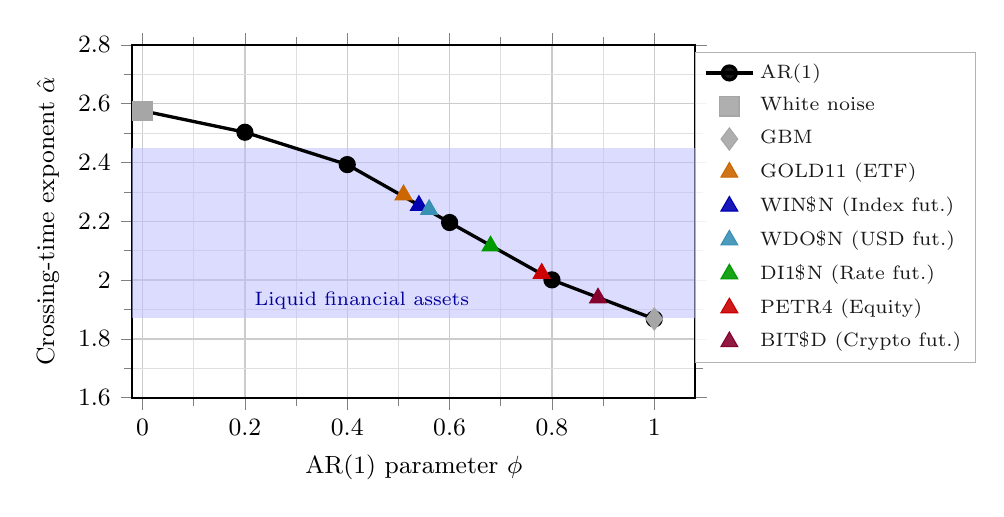
\begin{tikzpicture}
\begin{axis}[
  width  = 0.72\linewidth,
  height = 0.50\linewidth,
  xlabel = {AR(1) parameter $\phi$},
  ylabel = {Crossing-time exponent $\hat{\alpha}$},
  xmin = -0.02, xmax = 1.08,
  ymin = 1.60,  ymax = 2.80,
  xtick = {0, 0.2, 0.4, 0.6, 0.8, 1.0},
  ytick = {1.6, 1.8, 2.0, 2.2, 2.4, 2.6, 2.8},
  tick align = outside,
  minor tick num = 1,
  grid = both,
  grid style      = {line width=0.3pt, draw=gray!25},
  major grid style= {line width=0.5pt, draw=gray!40},
  axis line style = {line width=0.8pt},
  label style     = {font=\small},
  tick label style= {font=\small},
  legend style = {     at={(1.00,0.98)}, anchor=north west,
    font=\scriptsize, draw=gray!60,
    fill=white, fill opacity=0.9,
    row sep=1.5pt }, 
  legend cell align=left,
  clip = false,
]

% -------------------------------------------------------
% 1. Shaded band: liquid financial assets [1.87, 2.45]
% -------------------------------------------------------
\fill[blue!25, opacity=0.55]
  (axis cs:-0.02,1.87) rectangle (axis cs:1.08,2.45);
\node[font=\scriptsize, text=blue!60!black, anchor=west]
  at (axis cs:0.2, 1.93) {Liquid financial assets};

% -------------------------------------------------------
% 2. AR(1) measured curve
% -------------------------------------------------------
\addplot[
  color     = black,
  line width = 1.2pt,
  mark       = *,
  mark size  = 2.5pt,
  mark options = {fill=black},
  %error bars/y dir=both,
  %error bars/y explicit,
] coordinates {
  (0.0,  2.576) %+- (0, 0.351)
  (0.2,  2.503) %+- (0, 0.325)
  (0.4,  2.393) %+- (0, 0.277)
  (0.6,  2.196) %+- (0, 0.209)
  (0.8,  2.001) %+- (0, 0.151)
  (1.0,  1.868) %+- (0, 0.113)
};
\addlegendentry{AR(1)}

% -------------------------------------------------------
% 3. White-noise anchor
% -------------------------------------------------------
\addplot[
  only marks, mark=square*,
  mark size=3.5pt,
  mark options={fill=gray!70, draw=gray!70},
] coordinates { (0.0, 2.576) };
\addlegendentry{White noise}

% -------------------------------------------------------
% 4. GBM anchor
% -------------------------------------------------------
\addplot[
  only marks, mark=diamond*,
  mark size=4pt,
  mark options={fill=gray!70, draw=gray!70},
] coordinates { (1.0, 1.868) };
\addlegendentry{GBM}

% -------------------------------------------------------
% 5. Financial assets (phi_eff, alpha_M5)
% -------------------------------------------------------
% GOLD11  phi=0.51  alpha=2.290
\addplot[only marks, mark=triangle*, mark size=3.5pt,
  mark options={fill=orange!80!black,draw=orange!80!black}]
  coordinates { (0.51, 2.290) };
\addlegendentry{GOLD11 (ETF)}

% WIN$N   phi=0.54  alpha=2.254
\addplot[only marks, mark=triangle*, mark size=3.5pt,
  mark options={fill=blue!70!black,draw=blue!70!black}]
  coordinates { (0.54, 2.254) };
\addlegendentry{WIN\$N (Index fut.)}

% WDO$N   phi=0.56  alpha=2.240
\addplot[only marks, mark=triangle*, mark size=3.5pt,
  mark options={fill=cyan!70!black,draw=cyan!70!black}]
  coordinates { (0.56, 2.240) };
\addlegendentry{WDO\$N (USD fut.)}

% DI1$N   phi=0.68  alpha=2.116
\addplot[only marks, mark=triangle*, mark size=3.5pt,
  mark options={fill=green!60!black,draw=green!60!black}]
  coordinates { (0.68, 2.116) };
\addlegendentry{DI1\$N (Rate fut.)}

% PETR4   phi=0.78  alpha=2.023
\addplot[only marks, mark=triangle*, mark size=3.5pt,
  mark options={fill=red!80!black,draw=red!80!black}]
  coordinates { (0.78, 2.023) };
\addlegendentry{PETR4 (Equity)}

% BIT$D   phi=0.89  alpha=1.939
\addplot[only marks, mark=triangle*, mark size=3.5pt,
  mark options={fill=purple!70!black,draw=purple!70!black}]
  coordinates { (0.89, 1.939) };
\addlegendentry{BIT\$D (Crypto fut.)}

% -------------------------------------------------------
% 6. Horizontal dashed reference lines
% -------------------------------------------------------
%\addplot[dashed, gray, line width=0.7pt, forget plot]
%  coordinates {(-0.02,2.576)(1.08,2.576)};
%\node[font=\scriptsize, text=gray!80!black, anchor=west]
%  at (axis cs:1.03, 2.576) {$\alpha_{0}=2.58$};

%\addplot[dashed, gray, line width=0.7pt, forget plot]
%  coordinates {(-0.02,1.868)(1.08,1.868)};
%\node[font=\scriptsize, text=gray!80!black, anchor=west]
%  at (axis cs:1.03, 1.868) {$\alpha_{\mathrm{GBM}}=1.87$};

%\addplot[dashed, gray!50, line width=0.7pt, forget plot]
%  coordinates {(-0.02,2.00)(1.08,2.00)};
%\node[font=\scriptsize, text=gray!60!black, anchor=west]
%  at (axis cs:1.03, 2.00) {$\alpha=2$};

\end{axis}
\end{tikzpicture} \caption{Crossing-time exponent $\hat{\alpha}$ as a function of the AR(1)
parameter $\phi$. The curve interpolates monotonically between the
white-noise ceiling ($\alpha_{0}=2.576$, $\phi=0$) and the GBM floor
($\alpha_{\mathrm{GBM}}=1.868$, $\phi=1$). The blue shaded band
$[1.87,\,2.45]$ encompasses all liquid financial assets studied (coloured
markers, positioned at their effective $\phi_{\mathrm{eff}}$ obtained
by linear interpolation at the M5 $\hat{\alpha}$ value; Table~\ref{tab:phi_eff}).
Assets span $\phi_{\mathrm{eff}}\in[0.51,\,0.89]$, clustering closer
to the GBM limit than to white noise, with commodity and index instruments
at lower $\phi_{\mathrm{eff}}$ than equities and crypto-linked futures.}
\label{fig:alpha_phi} 
\end{figure}


\section{Window-Induced Correlations and Finite-Sample Distortions in MSD
Estimation}

The construction of the Hankel matrix $\mathbf{H}(\tau)$ over a sliding
window of size $W$ induces a non-trivial dependence structure in
the sequence of operators $\boldsymbol{K}(\tau)$. In particular,
successive matrices share $W-1$ observations, implying that $\boldsymbol{K}(\tau)$
and $\boldsymbol{K}(\tau+\ell)$ are statistically dependent for all
lags $\ell<W$. This dependence propagates to the cumulative process
\[
\boldsymbol{X}(\tau)=\int_{0}^{\tau}\boldsymbol{K}(s)\,ds,
\]
and, crucially, to its increments.

Consider the increment over a lag $\Delta\tau$, 
\[
\delta\boldsymbol{X}_{t}(\Delta\tau)=\boldsymbol{X}(t+\Delta\tau)-\boldsymbol{X}(t)=\sum_{s=t}^{t+\Delta\tau-1}\boldsymbol{K}(s).
\]
The empirical mean-square displacement (MSD) estimator is defined
as 
\[
\widehat{\Sigma}^{2}(\Delta\tau)=\frac{1}{N-\Delta\tau}\sum_{t=1}^{N-\Delta\tau}\|\delta\boldsymbol{X}_{t}(\Delta\tau)\|_{F}^{2}.
\]

Assuming stationarity, its expectation reads 
\[
\mathbb{E}\!\left[\widehat{\Sigma}^{2}(\Delta\tau)\right]=\mathbb{E}\!\left[\|\delta\boldsymbol{X}_{t}(\Delta\tau)\|_{F}^{2}\right],
\]
so that the estimator is unbiased with respect to the true MSD. Expanding
the squared norm yields 
\[
\Sigma^{2}(\Delta\tau)=\mathbb{E}\!\left[\|\delta\boldsymbol{X}_{t}(\Delta\tau)\|_{F}^{2}\right]=\sum_{i,j=0}^{\Delta\tau-1}\mathbb{E}\!\left[\langle\boldsymbol{K}(t+i),\boldsymbol{K}(t+j)\rangle_{F}\right].
\]

Introducing the autocovariance function 
\[
C_{K}(h)=\mathbb{E}\!\left[\langle\boldsymbol{K}(t+h),\boldsymbol{K}(t)\rangle_{F}\right],
\]
one obtains the standard representation 
\[
\Sigma^{2}(\Delta\tau)=\sum_{h=-(\Delta\tau-1)}^{\Delta\tau-1}(\Delta\tau-|h|)\,C_{K}(h),
\]
which explicitly shows that the MSD depends on the full temporal correlation
structure of $\boldsymbol{K}$.

The windowed construction implies that $C_{K}(h)$ remains non-negligible
up to lags of order $W$, defining an effective correlation horizon.
As a consequence, the MSD exhibits two distinct regimes: 
\[
\begin{cases}
\Delta\tau\lesssim W & \text{correlation-dominated regime},\\
\Delta\tau\gg W & \text{asymptotic regime}.
\end{cases}
\]

At short lags, the triangular weighting $(\Delta\tau-|h|)$ strongly
couples the MSD to short-range correlations in $\boldsymbol{K}$,
leading to deviations from the asymptotic scaling law. These deviations
are not due to a bias of the estimator itself, but rather reflect
the intrinsic correlation structure induced by the sliding window.

In addition, correlations between overlapping increments, 
\[
\mathrm{Cov}\!\left(\delta\boldsymbol{X}_{t}(\Delta\tau),\delta\boldsymbol{X}_{t+\ell}(\Delta\tau)\right)\neq0\quad\text{for }\ell<W,
\]
increase the variance of the estimator and induce finite-sample distortions
in the inferred scaling behaviour. In particular, positive correlations
tend to inflate the apparent growth of the MSD at short lags, while
negative correlations may produce an apparent subdiffusive regime.
These effects vanish asymptotically as $\Delta\tau\gg W$, where both
$C_{K}(h)$ and inter-increment correlations decay.

The magnitude of these finite-sample distortions is therefore controlled
by the window size $W$, which sets the scale of induced dependence.
In the main text, the choice $W=5L$ follows an optimization procedure
in which the structural exponent is empirically stable for multipliers
in the range $\{4L,5L,6L\}$ at the optimal embedding dimension $L_{\mathrm{opt}}$.
This choice effectively fixes the correlation horizon introduced by
the construction.

The estimation procedure explicitly mitigates these effects in two
ways. First, the base lag is chosen as $\Delta\tau_{\mathrm{opt}}$,
sufficiently larger than the elementary increment scale. Second, the
diffusion exponent is extracted from a log--log regression restricted
to the upper 70\% of lags, ensuring that the fit is performed within
the asymptotic regime $\Delta\tau\gg W$, where correlation-induced
distortions are negligible.

Under these conditions, the estimated exponent reflects the intrinsic
long-time dynamics of the process, rather than artefacts arising from
the sliding-window construction.

%Individual Asset Results
Proposed figures for supplementary
FigureS1. MSD of  (log-log) for all 14 assets, panels arranged by asset class. M5 and H1 shown on same axes. Reference lines  and  included.
FigureS2.  vs  for all 14 assets at M5 and H1. Vertical band at .
FigureS3.  vs  for all 14 assets.
FigureS4.  vs  (as Fig.3 of main text) for all 14 assets. Vertical band at .
FigureS5. MP bulk histogram (as Fig.1 of main text) for all 14 assets. Arranged in 5 panels by asset class.
Proposed tables for supplementary
TableS1. Complete table of exponents for all 13 assets: , , , , , and  for both M5 and H1.
TableS2. Bulk  error relative to MP law for all 13 assets and both timescales.
Robustness Checks
Sensitivity to .
Figure3 of the main text shows results for . All three ratios yield , confirming that  does not depend on  (i.e., on the number of delay vectors ). The value of  in the convergence region varies by  across , within the statistical uncertainty.
Sensitivity to regression window.
Varying the fraction of lags included in the regression from 50% to 90% (upper fraction) changes  by  for PETR4. The asymptotic plateau is clearly established by 60% and above.
Stationarity.
We verified stationarity of  over the 5-year observation window by computing the Augmented DickeyFuller test on the time series of  (total spectral mass),  (structural dimension), and  (spectral gap). All three quantities are stationary at the 1% level for all assets, consistent with the near-stationary assumption of the GLE.
Non-Gaussianity of bulk projections.
Although Eq.(11) of the main text predicts Gaussian projections onto bulk modes, the actual distributions exhibit excess kurtosis of , consistent with the Poisson jump term. This kurtosis is absorbed into the   error of the bulk histogram relative to the MP law.

\section{Relation to Existing Anomalous Diffusion Literature}

The generalized Langevin equation (GLE) framework employed here constitutes
a direct matrix-valued extension of the scalar GLE widely used in
the study of anomalous diffusion in complex systems. The key structural
difference lies in the block organisation of the memory kernel $\boldsymbol{\Gamma}$,
which enables the coexistence of distinct dynamical regimes within
orthogonal subspaces of the same operator process. In this sense,
normal and anomalous diffusion are not alternative descriptions, but
simultaneous projections of a higher-dimensional dynamics.

The connection with linear response theory is explicit. In analogy
with the Kubo formalism, the effective friction in the structural
subspace, 
\[
\gamma_{\mathrm{s}}^{\mathrm{eff}}=\hat{\Gamma}_{\mathrm{s}}(0),
\]
corresponds to the zero-frequency component of the memory kernel.
In the present construction, this quantity is estimated as 
\[
\gamma_{\mathrm{s}}(\tau)=\frac{1}{L}\mathrm{Tr}\big(\boldsymbol{\Gamma}_{\mathrm{s}}(\tau)\big),
\]
providing an operational definition of dissipation directly from the
data.

Within this framework, the squared Frobenius norm 
\[
\|\boldsymbol{K}\|_{F}^{2}=\mathrm{Tr}(\boldsymbol{K}^{\top}\boldsymbol{K})
\]
plays the role of an effective temperature, setting the amplitude
of fluctuations through the instantaneous spectral energy of the operator.
Although $\boldsymbol{K}$ is not a velocity in a strict mechanical
sense, it acts as the generator of increments of the integrated process
$\boldsymbol{X}(\tau)$, establishing a direct analogy with velocity-driven
diffusion. In this interpretation, $\|\boldsymbol{K}\|_{F}^{2}$ is
the natural counterpart of $\langle v^{2}\rangle$ in classical diffusion
theory.

This analogy leads to a matrix-valued Einstein relation for the structural
subspace, 
\[
D_{\mathrm{s}}=\frac{\|\boldsymbol{K}_{\mathrm{s}}\|_{F}^{2}}{\gamma_{\mathrm{s}}^{\mathrm{eff}}},
\]
which expresses diffusion as the ratio between fluctuation intensity
and effective dissipation. Importantly, both quantities are endogenously
determined by the data through the same operator construction, in
contrast with standard approaches where noise and memory kernels are
specified a priori.

From this perspective, the scalar diffusion coefficient emerges as
a reduced description of an underlying operator-valued transport process.
The present framework therefore provides a natural bridge between
matrix GLE formulations and classical anomalous diffusion theory,
while extending the latter to settings where multiple dynamical regimes
coexist within a single observable structure.

\bibliographystyle{naturemag}
\bibliography{spectral_dynamics}

\end{document}
